\documentclass{article}

\usepackage{amsmath, amssymb}
\usepackage{graphicx}

\title{Time and Distance}
\author{Richard Feynman}
\begin{document}

	\maketitle

	\section{Motion}

	In this chapter we shall consider some aspects of the concepts of time and distance. It has been emphasized earlier that physics, as do all the sciences, depends on observation. One might also say that the development of the physical sciences to their present form has depended to a large extent on the emphasis which has been placed on the making of quantitative observations. Only with quantitative observations can one arrive at quantitative relationships, which are the heart of physics.\\

	Many people would like to place the beginnings of physics with the work done 350 years ago by Galileo, and to call him the first physicist. Until that time, the study of motion had been a philosophical one based on arguments that could be thought up in one’s head. Most of the arguments had been presented by Aristotle and other Greek philosophers, and were taken as “proven.” Galileo was skeptical, and did an experiment on motion which was essentially this: He allowed a ball to roll down an inclined trough and observed the motion. He did not, however, just look; he measured how far the ball went in how long a time.\\

	The way to measure a distance was well known long before Galileo, but there were no accurate ways of measuring time, particularly short times. Although he later devised more satisfactory clocks (though not like the ones we know), Galileo’s first experiments on motion were done by using his pulse to count off equal intervals of time. Let us do the same.\\

	We may count off beats of a pulse as the ball rolls down the track: “one … two … three … four … five … six … seven … eight …” We ask a friend to make a small mark at the location of the ball at each count; we can then measure the distance the ball travelled from the point of release in one, or two, or three, etc., equal intervals of time. Galileo expressed the result of his observations in this way: if the location of the ball is marked at 1, 2, 3, 4, … units of time from the instant of its release, those marks are distant from the starting point in proportion to the numbers 1, 4, 9, 16, … Today we would say the distance is proportional to the square of the time: 

	\begin{figure}[h]
	\centering
		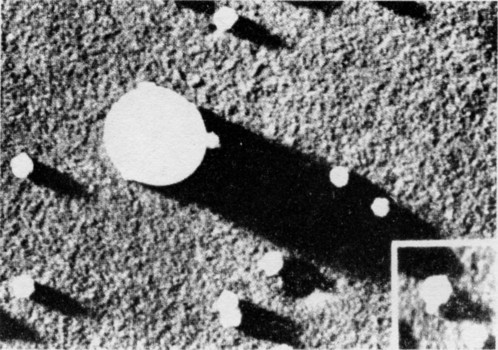
\includegraphics{img1.png}
		\caption{A ball rolls down an inclined track}
		\label{Fi: Galaxia}
	\end{figure}

	The study of motion, which is basic to all of physics, treats with the questions: where? and when?

	\section{Time}


	Let us consider first what we mean by time. What is time? It would be nice if we could find a good definition of time. Webster defines “a time” as “a period,” and the latter as “a time,” which doesn’t seem to be very useful. Perhaps we should say: “Time is what happens when nothing else happens.” Which also doesn’t get us very far. Maybe it is just as well if we face the fact that time is one of the things we probably cannot define (in the dictionary sense), and just say that it is what we already know it to be: it is how long we wait!.\\

	What really matters anyway is not how we define time, but how we measure it. One way of measuring time is to utilize something which happens over and over again in a regular fashion—something which is periodic. For example, a day. A day seems to happen over and over again. But when you begin to think about it, you might well ask: “Are days periodic; are they regular? Are all days the same length?” One certainly has the impression that days in summer are longer than days in winter. Of course, some of the days in winter seem to get awfully long if one is very bored. You have certainly heard someone say, “My, but this has been a long day!”.\\

	It does seem, however, that days are about the same length on the average. Is there any way we can test whether the days are the same length—either from one day to the next, or at least on the average? One way is to make a comparison with some other periodic phenomenon. Let us see how such a comparison might be made with an hour glass. With an hour glass, we can “create” a periodic occurrence if we have someone standing by it day and night to turn it over whenever the last grain of sand runs out.\\

	We could then count the turnings of the glass from each morning to the next. We would find, this time, that the number of “hours” (i.e., turnings of the glass) was not the same each “day.” We should distrust the sun, or the glass, or both. After some thought, it might occur to us to count the “hours” from noon to noon. (Noon is here defined not as 12:00 o’clock, but that instant when the sun is at its highest point.) We would find, this time, that the number of “hours” each day is the same.\\

	We now have some confidence that both the “hour” and the “day” have a regular periodicity, i.e., mark off successive equal intervals of time, although we have not proved that either one is “really” periodic. Someone might question whether there might not be some omnipotent being who would slow down the flow of sand every night and speed it up during the day. Our experiment does not, of course, give us an answer to this sort of question. All we can say is that we find that a regularity of one kind fits together with a regularity of another kind. We can just say that we base our definition of time on the repetition of some apparently periodic event.\\

	\section{Short times}

	We should now notice that in the process of checking on the reproducibility of the day, we have received an important by-product. We have found a way of measuring, more accurately, fractions of a day. We have found a way of counting time in smaller pieces. Can we carry the process further, and learn to measure even smaller intervals of time?\\

	Galileo decided that a given pendulum always swings back and forth in equal intervals of time so long as the size of the swing is kept small. A test comparing the number of swings of a pendulum in one “hour” shows that such is indeed the case. We can in this way mark fractions of an hour. If we use a mechanical device to count the swings—and to keep them going—we have the pendulum clock of our grandfathers.\\

	Let us agree that if our pendulum oscillates 3600 times in one hour (and if there are 24 such hours in a day), we shall call each period of the pendulum one “second.” We have then divided our original unit of time into approximately 105 parts. We can apply the same principles to divide the second into smaller and smaller intervals. It is, you will realize, not practical to make mechanical pendulums which go arbitrarily fast, but we can now make electrical pendulums, called oscillators, which can provide a periodic occurrence with a very short period of swing. In these electronic oscillators it is an electrical current which swings to and fro, in a manner analogous to the swinging of the bob of the pendulum.\\

	We can make a series of such electronic oscillators, each with a period 10 times shorter than the previous one. We may “calibrate” each oscillator against the next slower one by counting the number of swings it makes for one swing of the slower oscillator. When the period of oscillation of our clock is shorter than a fraction of a second, we cannot count the oscillations without the help of some device which extends our powers of observation. One such device is the electron-beam oscilloscope, which acts as a sort of microscope for short times. This device plots on a fluorescent screen a graph of electrical current (or voltage) versus time. By connecting the oscilloscope to two of our oscillators in sequence, so that it plots a graph first of the current in one of our oscillators and then of the current in the other, we get two graphs like those shown in Fig. 5–2. We can readily determine the number of periods of the faster oscillator in one period of the slower oscillator.\\

	\begin{figure}[h]
	\centering
		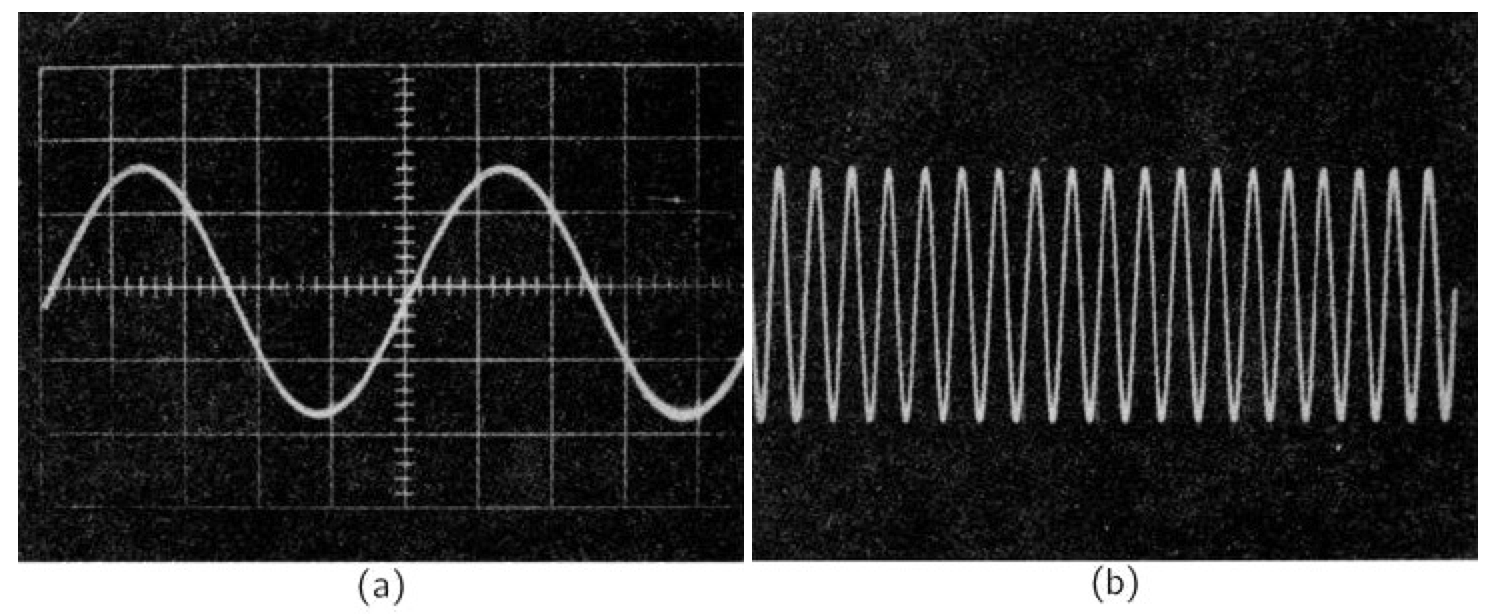
\includegraphics{img2.png}
		\caption{Two views of an oscilloscope screen. In (a) the oscilloscope is connected to one oscillator, in (b) it is connected to an oscillator with a period one-tenth as long.}
		\label{Fi: Galaxia}
	\end{figure}


\end{document}